\documentclass[aspectratio=169,11pt]{beamer}
\usetheme[progressbar=frametitle,numbering=fraction,block=fill]{metropolis}
\usepackage[T1]{fontenc}
\usepackage[sfdefault,lining]{FiraSans}
\usepackage[scale=0.85,lining]{FiraMono}
\usepackage{amsmath,amssymb,bm,mathtools}
\usepackage{booktabs,array}
\usepackage{listings}
\usepackage{tikz}
\usetikzlibrary{arrows.meta,positioning,shapes.misc}
\graphicspath{{../images/}}

% ---------------- palette ----------------
\definecolor{navy}{HTML}{1B2A41}
\definecolor{teal}{HTML}{1F7A8C}
\definecolor{sand}{HTML}{F4F1EA}
\definecolor{ink}{HTML}{2B2B2B}
\definecolor{muted}{HTML}{6B6B6B}
\definecolor{orange}{HTML}{D9622B}
\setbeamercolor{frametitle}{bg=navy,fg=white}
\setbeamercolor{progress bar}{fg=teal,bg=navy!25}
\setbeamercolor{title separator}{fg=teal}
\setbeamercolor{title}{fg=navy}
\setbeamercolor{subtitle}{fg=teal}
\setbeamercolor{normal text}{fg=ink,bg=white}
\setbeamercolor{alerted text}{fg=orange}
\setbeamercolor{block title}{bg=teal!15,fg=navy}
\setbeamercolor{block body}{bg=sand}
\setbeamercolor{background canvas}{bg=white}
\setbeamertemplate{bibliography item}[text]
\setbeamerfont{bibliography item}{size=\scriptsize}
\setbeamerfont{bibliography entry author}{size=\scriptsize}
\setbeamerfont{bibliography entry title}{size=\scriptsize}
\setbeamerfont{bibliography entry location}{size=\scriptsize}
\setbeamerfont{bibliography entry note}{size=\scriptsize}
\setbeamercolor{bibliography entry author}{fg=ink}
\setbeamercolor{bibliography entry note}{fg=ink}
\setbeamerfont{frametitle}{size=\large}
\setbeamerfont{title}{size=\huge,series=\bfseries}
\setbeamerfont{block title}{size=\small}

\newcommand{\Om}{\hat{\Omega}}
\newcommand{\dd}{\mathrm{d}}
\newcommand{\kron}{\otimes}
\newcommand{\pp}{{\bm p^{+}}}
\newcommand{\pmn}{{\bm p^{-}}}
\newcommand{\diag}{\operatorname{diag}}

\lstset{language=Python,basicstyle=\ttfamily\tiny,columns=fullflexible,keepspaces=true,
        keywordstyle=\color{navy}\bfseries,commentstyle=\color{muted},stringstyle=\color{teal},
        showstringspaces=false,backgroundcolor=\color{sand},frame=none,xleftmargin=3pt,xrightmargin=3pt,
        aboveskip=2pt,belowskip=2pt,upquote=true}

\title{TT Slab Neutron Transport}
\subtitle{Tensor-train discrete ordinates in slab geometry, verified against OpenMC}
\author{}   % add name
\institute{}
\date{\today}

\begin{document}

%==========================================================================================
\maketitle

%==========================================================================================
\begin{frame}{Problem definition}
\small
Multigroup, time-dependent transport in a slab $z\in[0,L]$, full angle $\Om=\Om(\mu,\varphi)$, $g=1,\dots,G$:
\begin{equation*}
\Big(\frac{1}{v_g}\partial_t+\mu\,\partial_z+\sigma_{t,g}(z)\Big)\psi_g
=\sum_{g'}\int_{4\pi}\sigma_{s,g'\to g}(z,\Om\cdot\Om')\,\psi_{g'}(z,\Om',t)\,\dd\Om'+Q_g(z,\Om,t)
\end{equation*}
\vspace{-1ex}
\begin{columns}[T,onlytextwidth]
\column{0.44\textwidth}
\begin{block}{Boundary and initial conditions}
\vspace{-2ex}
\begin{align*}
\psi_g(0,\Om,t)&=\psi^{\mathrm L}_g(\Om,t), && \mu>0\\[-2pt]
\psi_g(L,\Om,t)&=\psi^{\mathrm R}_g(\Om,t), && \mu<0\\[-2pt]
\psi_g(z,\Om,0)&=\psi^{0}_g(z,\Om)
\end{align*}
\end{block}
\column{0.52\textwidth}
\begin{block}{$C$ materials, $P_\Lambda$ scattering kernel}
\vspace{-2ex}
\begin{gather*}
\sigma_{t,g}(z)=\textstyle\sum_{c=1}^{C}\mathbf 1_c(z)\,\sigma^c_{t,g}\\[-2pt]
\sigma^c_{s,g'\to g}(\mu_0)=\sum_{l=0}^{\Lambda}\frac{2l+1}{4\pi}\,\sigma^{l,c}_{s,g'\to g}\,P_l(\mu_0)
\end{gather*}
\end{block}
\end{columns}
\vspace{1ex}
{\footnotesize With real spherical harmonics, $P_l(\Om\cdot\Om')=\frac{4\pi}{2l+1}\sum_m Y_{lm}(\Om)Y_{lm}(\Om')$: energy enters only through the matrices $\Sigma^{l,c}=[\sigma^{l,c}_{s,g'\to g}]$.}
\end{frame}

%==========================================================================================

%==========================================================================================
\begin{frame}{Phase-space discretization}
\centering
\footnotesize
\renewcommand{\arraystretch}{1.1}
\begin{tabular}{@{}lccccc@{}}
\toprule
 & $z$ & $\mu$ & $\varphi$ & $E$ & $t$\\
\midrule
method & upwind DG ($p$)~\cite{ReedHill} & Gauss--Legendre & trapezoid & multigroup & backward Euler\\
unknowns & $N_z(p+1)$ & $N_\mu$ & $N_\varphi$ & $G$ & $N_t$\\
\bottomrule
\end{tabular}
\vspace{0.8ex}

\raggedright
\footnotesize
\begin{align*}
\mathcal A={}&\sum\nolimits_{c=1}^{C}M_c\kron\Big[\underbrace{I\kron I\kron\Sigma^c_t\kron I}_{\text{reaction}}
\;-\;\underbrace{\sum\nolimits_{l=0}^{\Lambda}K_l\kron\Sigma^{l,c}\kron I}_{\text{scattering}}\Big]
\\[-1ex]
&+\underbrace{M\kron I\kron I\kron V^{-1}\kron D_t}_{\text{time derivative}}
\;+\;\underbrace{\sum\nolimits_{\pm}\big(U^{\pm}-\mathsf S\big)\kron D^{\pm}_\mu\kron I\kron I\kron I}_{\text{streaming (upwind DG)}}\\[-0.3ex]
F={}&\underbrace{\bm Q_z\kron\bm Q_\mu\kron\bm Q_\varphi\kron\bm Q_E\kron\bm Q_t}_{\text{source}}
\;+\;\underbrace{\tfrac{1}{\Delta t}\,\bm\Psi^0_z\kron\bm\Psi^0_\mu\kron\bm\Psi^0_\varphi\kron V^{-1}\bm\Psi^0_E\kron\bm e_1}_{\text{initial condition}}\\[-1ex]
&+\underbrace{\big(\bm e_1\kron\pmn\big)\kron D^{+}_\mu\bm b^{L}_\mu\kron\bm b^{L}_\varphi\kron\bm b^{L}_E\kron\bm b^{L}_t
\;-\;\big(\bm e_{N_z}\kron\pp\big)\kron D^{-}_\mu\bm b^{R}_\mu\kron\bm b^{R}_\varphi\kron\bm b^{R}_E\kron\bm b^{R}_t}_{\text{boundary conditions (inflow at }z=0,\ z=L)}
\end{align*}
\end{frame}

%==========================================================================================
\begin{frame}[fragile]{The \texttt{SlabTransport} class}
\begin{lstlisting}[basicstyle=\ttfamily\scriptsize]
class SlabTransport:
    def __init__(self, N_z, p, L_z, N_mu, N_phi,
                 sigma_t,          # (G,) homogeneous | (C, G) table: C materials
                 sigma_s,          # list of (G, G) | (C, L+1, G, G), row = incoming group
                 v=None, E_edges=None, N_t=1, T=1.0, steady_state=False,
                 azimuthal_symmetry=False, mode="frw",    # "frw" | "adj"
                 region_map=None,  # chi: (N_z, C) 0/1, one material per cell; required with (C, G)
                 N_recon=3, K_round_prec=1e-12, A_round_prec=1e-13)
\end{lstlisting}
\vspace{1ex}
\begin{columns}[T,onlytextwidth]
\column{0.56\textwidth}
\begin{lstlisting}[basicstyle=\ttfamily\scriptsize]
set_source([q_z, q_mu, q_phi, q_E, q_t])
set_IC([ic_z, ic_mu, ic_phi, ic_E])
set_BC_left([bc_mu, bc_phi, bc_E, bc_t])  # + right
construct_tt_operator(); construct_tt_rhs()
run_amen(nswp=40, eps=1e-6, kickrank=4)
compute_scalar_flux()   # TT over (z_r, g, t)
inner(F)                # <psi, f>: responses
check_region_map(chi, N_z, C)  # in __init__
\end{lstlisting}
\column{0.40\textwidth}
\footnotesize
\begin{block}{Design}
\scriptsize
\begin{itemize}\setlength\itemsep{1pt}
\item $C$ materials, steady or transient, forward or adjoint
\item nuclear data in, physical flux out
\item adjoint: angle--time mirror of the forward problem
\item flux and responses stay in TT format
\end{itemize}
\end{block}
\end{columns}
\end{frame}

%==========================================================================================
\begin{frame}{Semi-analytical benchmark: infinite medium (after Ganapol)}
\begin{columns}[T,onlytextwidth]
\column{0.56\textwidth}
\centering
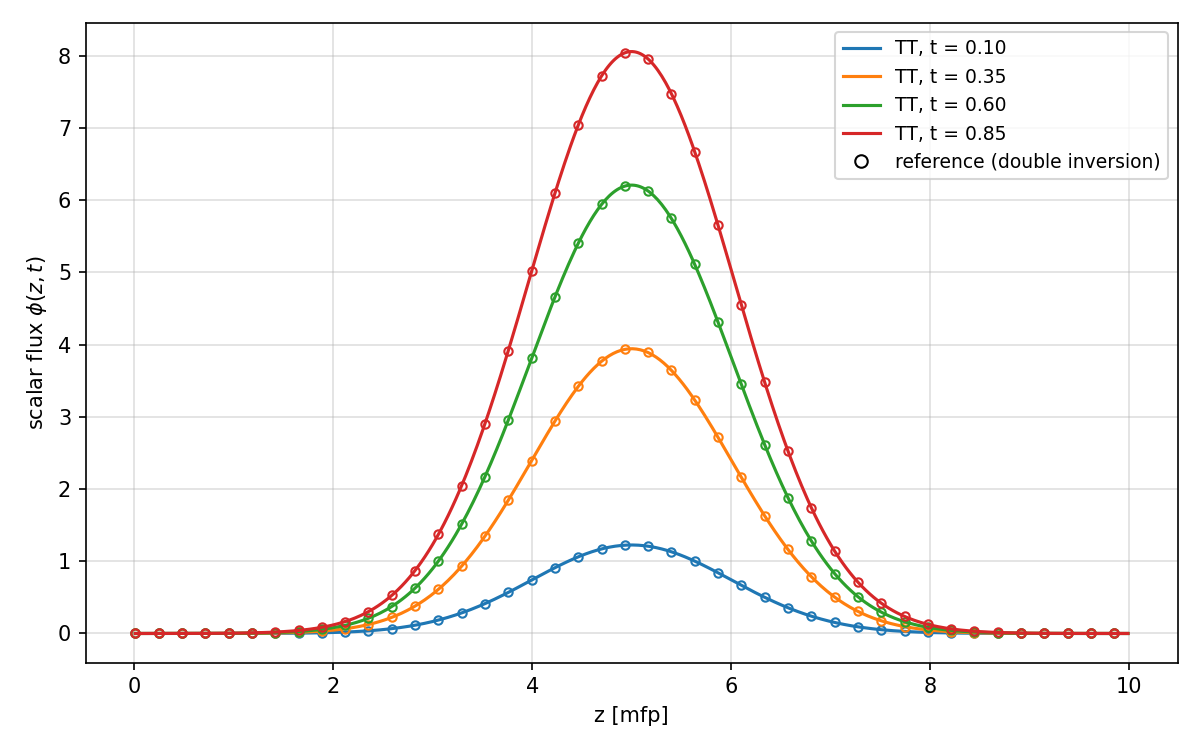
\includegraphics[width=\linewidth]{infinite_medium_gaussian.png}

\scriptsize Reference: Laplace--Fourier transform solution~\cite{DM}, double numerical inversion~\cite{Ganapol,DA}.
\column{0.40\textwidth}
\footnotesize
One group, isotropic scattering, $c=0.5$; source $e^{-\alpha z^2}e^{-\lambda t}$ ($\alpha=0.5$, $\lambda=0.1$), zero IC; slab $L=10$ mfp, $T=1$.
$N_z=512$, $p=1$, $N_\mu=N_\varphi=256$, $N_t=1024$.
\vspace{1ex}

\scriptsize
\begin{tabular*}{\linewidth}{@{}l@{\extracolsep{\fill}}r@{}}
\toprule
rel.\ $L^2$ error, $t=0.1\dots0.85$ & $5.6$--$3.2\cdot10^{-4}$\\
\midrule
operator ranks & $[6,6,6,6]$\\
solution ranks & $[13,8,8,8]$\\
TT compression & $1.7\cdot10^{-6}$\\
AMEn $\varepsilon$, nswp, kickrank & $10^{-6}$, 20, 4\\
sweeps, final Maxres & 6, \ $3.8\cdot10^{-7}$\\
time & 165 s\\
\bottomrule
\end{tabular*}
\vspace{1ex}

\footnotesize $6.9\cdot10^{10}$ unknowns stored in $5.8\cdot10^4$ TT entries.
\end{columns}
\end{frame}

%==========================================================================================
\begin{frame}{Cross sections from OpenMC: CE run $\to$ MGXS $\to$ TT}
\begin{columns}[c,onlytextwidth]
\column{0.41\textwidth}
\centering
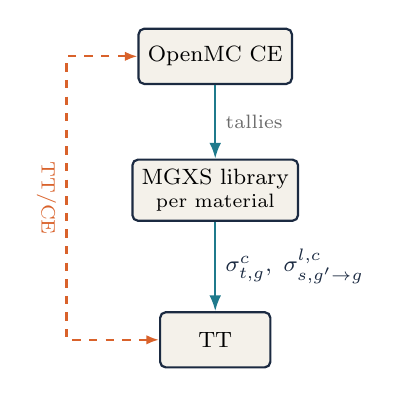
\begin{tikzpicture}[
  box/.style={rectangle,rounded corners=2pt,draw=navy,fill=sand,thick,minimum height=7mm,minimum width=14mm,
              align=center,font=\footnotesize},
  arr/.style={-{Latex[length=2mm]},thick,teal},
  cmp/.style={{Latex[length=1.6mm]}-{Latex[length=1.6mm]},dashed,orange,thick},
  lab/.style={font=\scriptsize,text=muted,align=center}]
\node[box] (ce) at (0,0) {OpenMC CE};
\node[box] (xs) at (0,-1.7) {MGXS library\\[-1pt]\scriptsize per material};
\node[box] (tt) at (0,-3.6) {TT};
\draw[arr] (ce) -- node[lab,right]{tallies} (xs);
\draw[arr] (xs) -- node[lab,right,text=navy,font=\footnotesize]{$\sigma^c_{t,g},\ \sigma^{l,c}_{s,g'\to g}$} (tt);
\draw[cmp] (ce.west) -- ++(-0.9,0) |- node[lab,sloped,below,pos=0.25,text=orange]{TT/CE} (tt.west);
\end{tikzpicture}

\vspace{1ex}\scriptsize OpenMC~\cite{OpenMC}, \texttt{openmc.mgxs}~\cite{MGXS}
\column{0.56\textwidth}
\scriptsize\raggedright
\renewcommand{\arraystretch}{1.3}
\begin{tabular}{@{}>{\raggedright\arraybackslash}p{0.17\linewidth}>{\raggedright\arraybackslash}p{0.36\linewidth}>{\raggedright\arraybackslash}p{0.41\linewidth}@{}}
\toprule
 & \textbf{CE run} & \textbf{TT}\\
\midrule
energy & continuous, pointwise ENDF/B; thermal $S(\alpha,\beta)$ & $G$ bins; spectrum inside a bin lost\\
cross sections & exact at each energy & $\sigma_g=\int_g\sigma\phi\,/\int_g\phi$ with the CE flux, averaged over each material\\
scattering angle & exact laws & Legendre moments $\sigma^{l}_{s,g'\to g}$, $l\le\Lambda$\\
space & flux tallied on $N_z$ cells & same cells\\
\bottomrule
\end{tabular}
\end{columns}
\end{frame}

%==========================================================================================
\begin{frame}{Graphite slab, $P_{20}$: group collapse, 16 to 256 groups}
\begin{columns}[T,onlytextwidth]
\column{0.58\textwidth}
\centering
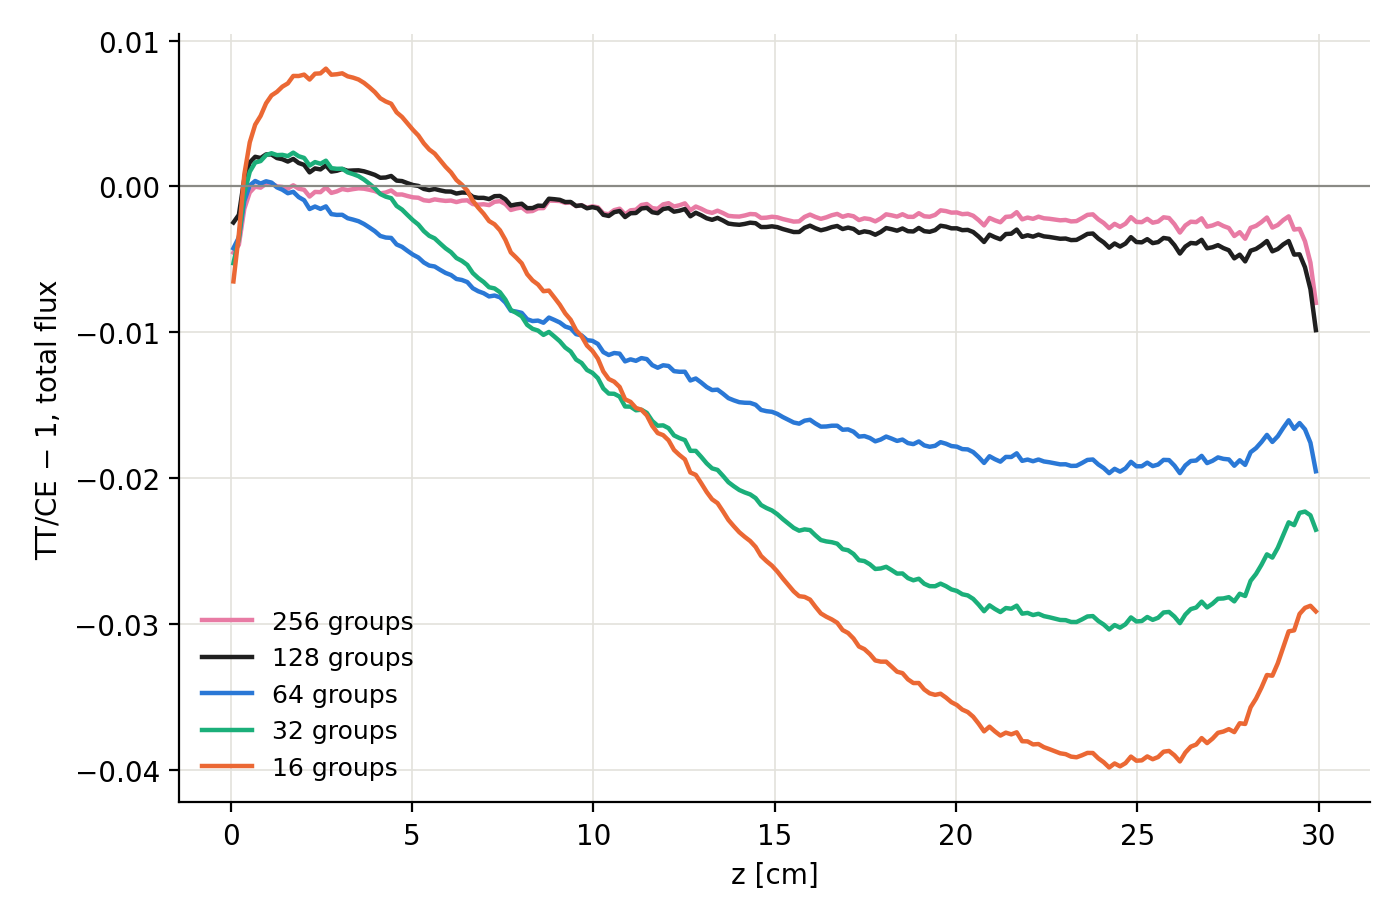
\includegraphics[width=\linewidth]{graphite_groups_tt_ce.png}
\column{0.38\textwidth}
\footnotesize
30 cm graphite, 2 MeV beam; $N_z=200$, $p=1$, $N_\mu=24$. 128 and 256 groups tallied directly, 16--64 collapsed from 128.
\vspace{1ex}

\scriptsize
\begin{tabular*}{\linewidth}{@{}r@{\extracolsep{\fill}}rrr@{}}
\toprule
$G$ & TT/CE int. & TT compr. & sweeps\\
\midrule
16 & $-1.71\%$ & $0.175$ & 13\\
32 & $-1.58\%$ & $0.132$ & 39\\
64 & $-1.18\%$ & $0.126$ & 40\\
128 & $-0.17\%$ & $0.096$ & 40\\
256 & $-0.16\%$ & $0.080$ & 40\\
\midrule
\multicolumn{4}{@{}l@{}}{AMEn $\varepsilon=10^{-7}$, nswp $=40$, kickrank $=4$}\\
\bottomrule
\end{tabular*}
\end{columns}
\end{frame}

%==========================================================================================
\begin{frame}{Graphite slab, 128 groups, $P_{20}$}
\begin{columns}[T,onlytextwidth]
\column{0.56\textwidth}
\centering
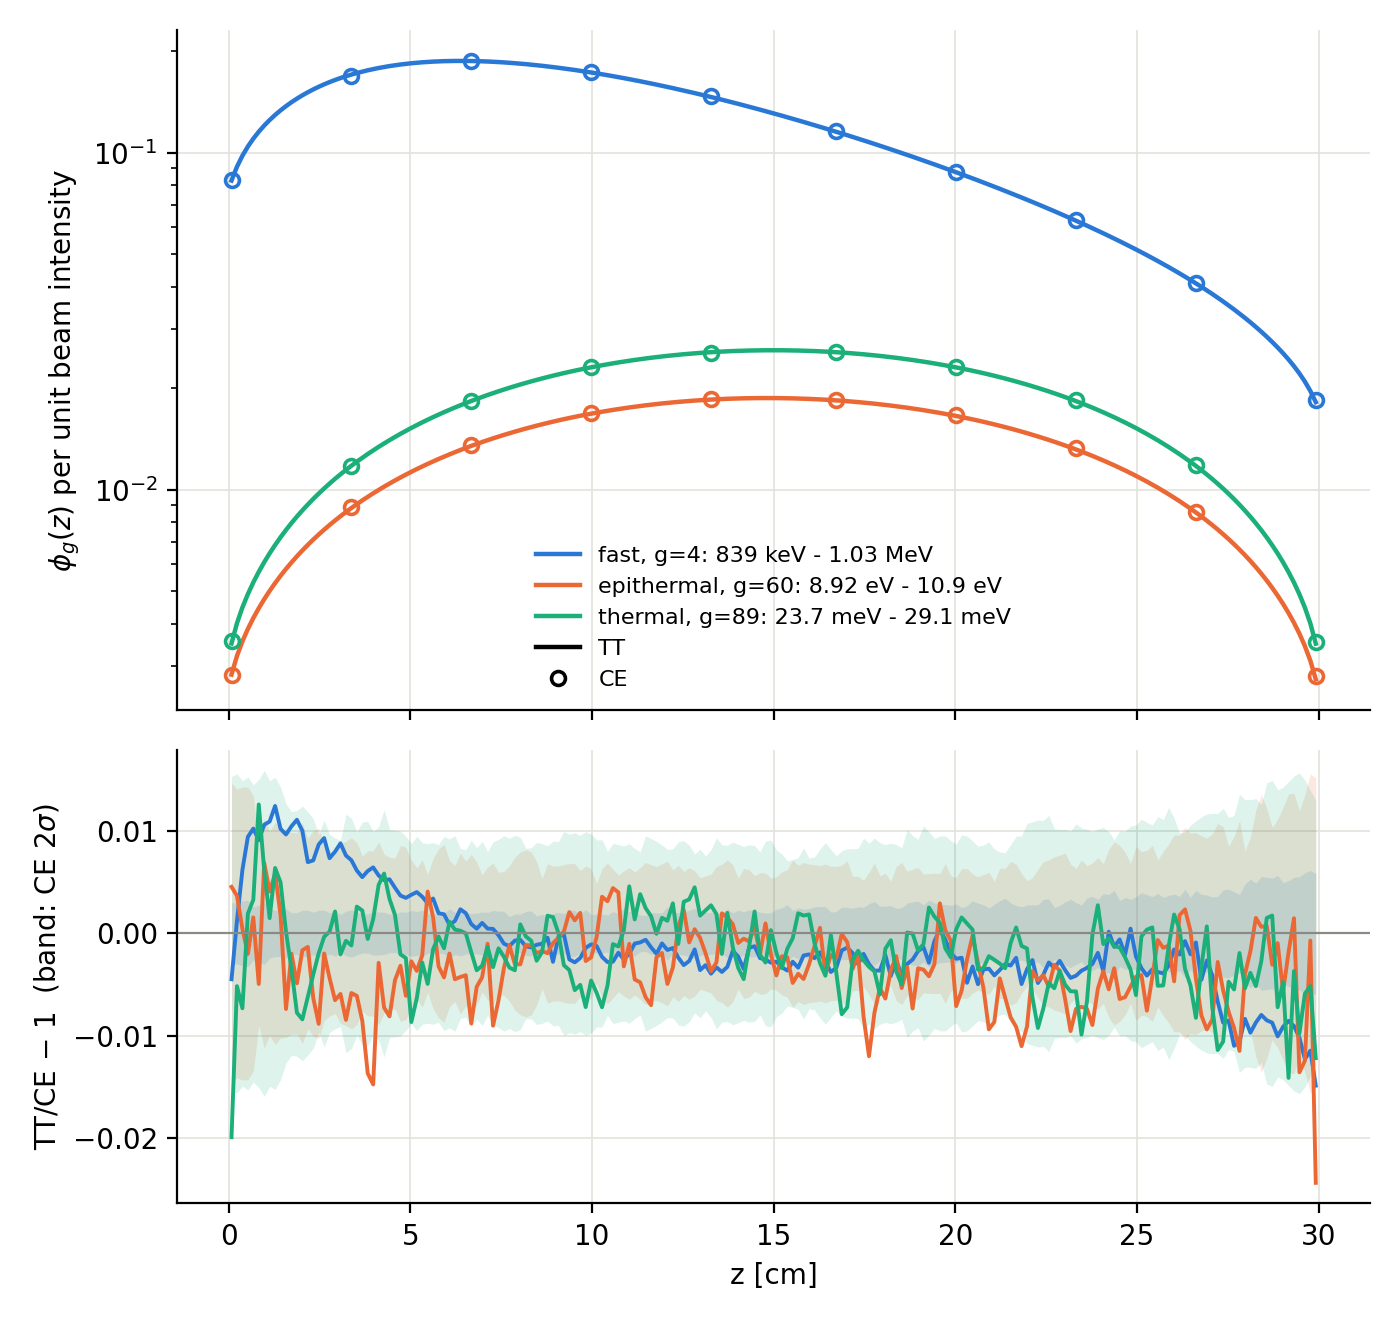
\includegraphics[height=0.80\textheight]{graphite_g128_tt_ce.png}
\column{0.40\textwidth}
\footnotesize
30 cm graphite, 2 MeV beam; $N_z=200$, $p=1$, $N_\mu=24$, azimuthal symmetry.
\vspace{1ex}

\scriptsize
\begin{tabular*}{\linewidth}{@{}l@{\extracolsep{\fill}}r@{}}
\toprule
TT/CE, integrated & \\
\quad total flux & $-0.17\%$\\
% \quad fast ($>0.1$ MeV) & $-0.07\%$\\
% \quad epithermal & $-0.25\%$\\
% \quad thermal ($<1$ eV) & $-0.30\%$\\
\quad $g=4$ (1 MeV) & $+0.01\%$\\
\quad $g=60$ (10 eV) & $-0.33\%$\\
\quad $g=89$ (26 meV) & $-0.17\%$\\
\midrule
operator ranks & $[5,25,25,5]$\\
solution ranks & $[53,66,68,1]$\\
TT compression & $0.096$\\
AMEn $\varepsilon$, nswp, kickrank & $10^{-7}$, 40, 4\\
sweeps, final residual & 40, \ $8.0\cdot10^{-7}$\\
\bottomrule
\end{tabular*}
\end{columns}
\end{frame}

%==========================================================================================
\begin{frame}{Graphite + 2 cm He-3 detector, 128 groups, $P_{20}$}
\begin{columns}[T,onlytextwidth]
\column{0.56\textwidth}
\centering
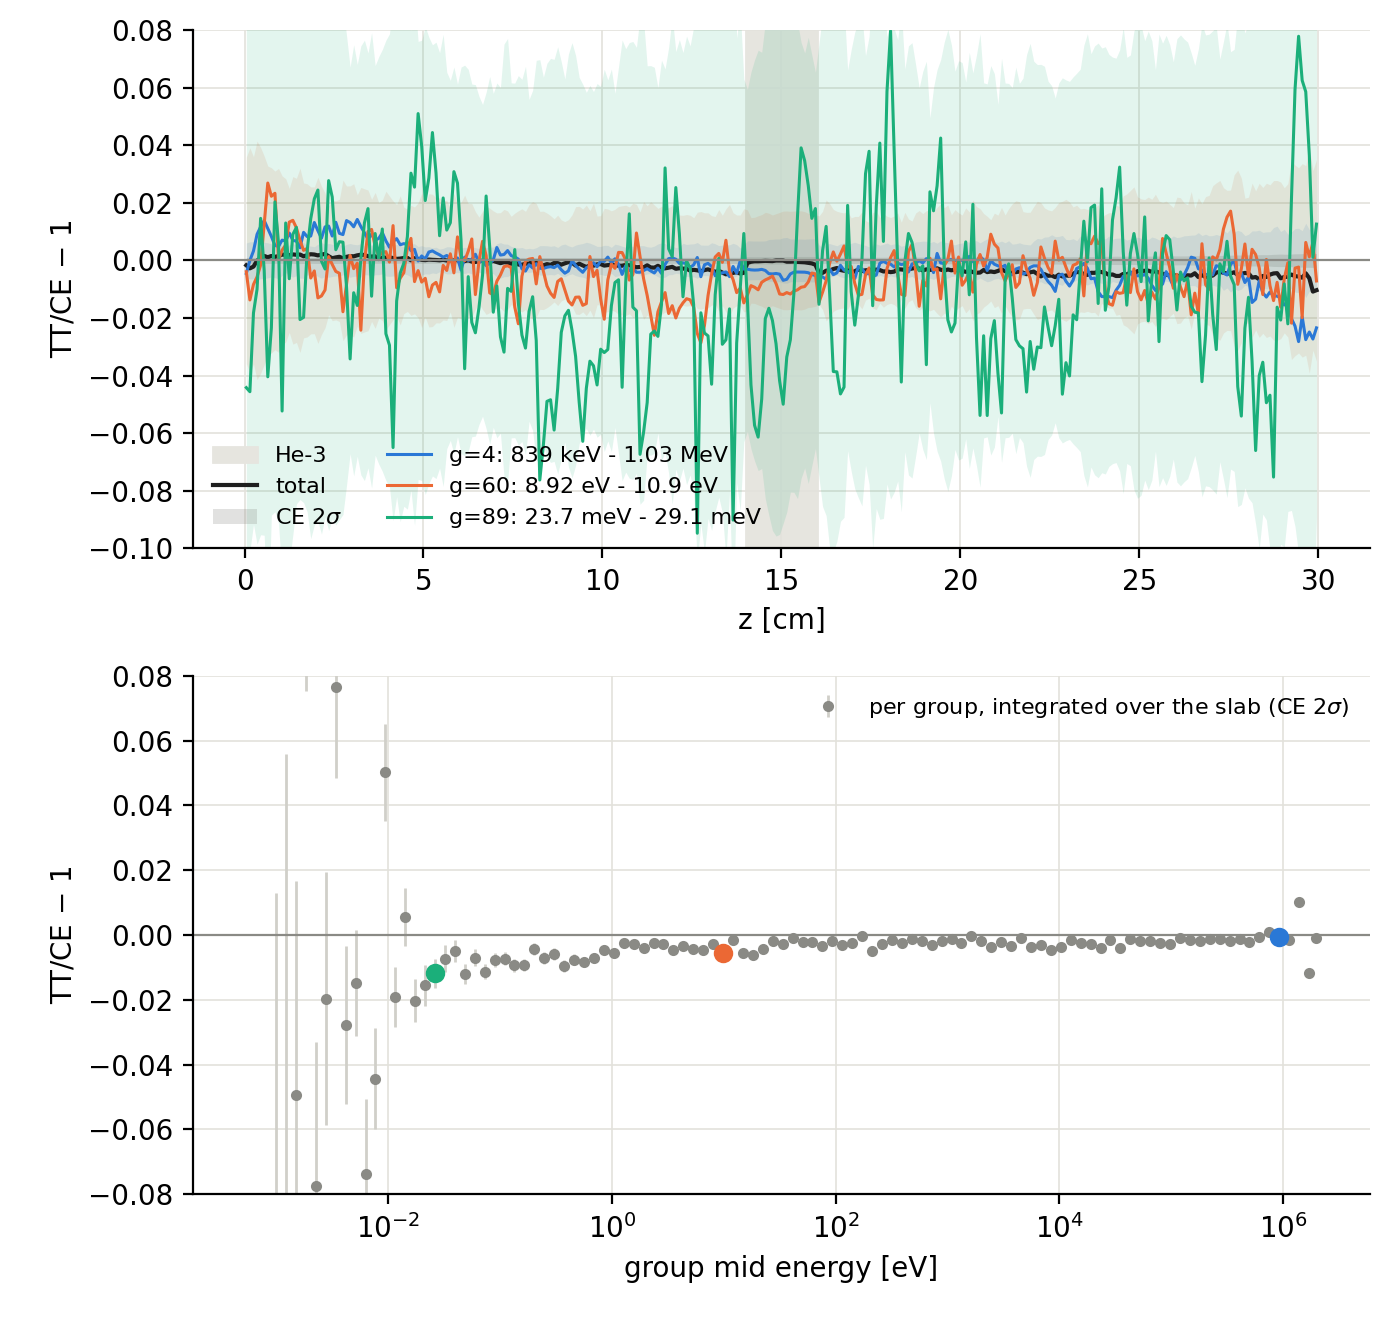
\includegraphics[height=0.80\textheight]{graphite_he3_tt_ce.png}
\column{0.40\textwidth}
\footnotesize
He-3 gas at $z\in[14,16]$ cm: $C=2$, MGXS per material; $N_z=300$, $p=1$, $N_\mu=24$.
\vspace{1ex}

\scriptsize
\begin{tabular*}{\linewidth}{@{}l@{\extracolsep{\fill}}r@{}}
\toprule
TT/CE, integrated & \\
\quad total flux & $-0.19\%$\\
\quad $g=4$ (1 MeV) & $-0.06\%$\\
\quad $g=60$ (10 eV) & $-0.55\%$\\
\quad $g=89$ (26 meV) & $-1.18\%$\\
\quad He-3 absorptions $R$ & \alert{$-0.20\%$}\\
\midrule
TT compression & $0.043$\\
AMEn $\varepsilon$, round & $10^{-5}$, $10^{-6}$\\
AMEn nswp, kickrank & 40, 4\\
sweeps & 20\\
\bottomrule
\end{tabular*}

\end{columns}
\end{frame}

%==========================================================================================

%==========================================================================================
\begin{frame}{Summary and outlook}
\begin{columns}[T,onlytextwidth]
\column{0.48\textwidth}
\begin{block}{Progress}
\small
\begin{itemize}
\item Real cross-section data: total $\sigma_{t,g}$ and scattering $\sigma^{l}_{s,g'\to g}$ from OpenMC
\item Semi-analytical time-dependent benchmark, after Ganapol~\cite{Ganapol}
\item Heterogeneous media: cell masks $\chi$, one operator term per material
\item Good agreement with OpenMC on stationary problems
\end{itemize}
\end{block}
\column{0.48\textwidth}
\begin{block}{Future developments}
\small
\begin{itemize}
\item Compression and rank growth with many cells
\item Time-dependent Monte Carlo benchmark
\item Adjoint treatment (time reversal~\cite{Acosta})
\item Extension to 3D space
\end{itemize}
\end{block}
\end{columns}
\end{frame}

%==========================================================================================
\begin{frame}{References}
\scriptsize
\begin{thebibliography}{9}
\setlength{\itemsep}{0pt}\scriptsize
\bibitem{ReedHill} W.~H. Reed and T.~R. Hill, Triangular mesh methods for the neutron transport equation, Los Alamos Scientific Laboratory report LA-UR-73-479 (1973).
\bibitem{HG} L.~G. Henyey and J.~L. Greenstein, Diffuse radiation in the galaxy, \emph{Astrophys.\ J.} 93 (1941) 70--83.
\bibitem{DM} J.~J. Duderstadt and W.~R. Martin, \emph{Transport Theory}, Wiley, 1979.
\bibitem{Ganapol} B.~D. Ganapol, \emph{Analytical Benchmarks for Nuclear Engineering Applications}, OECD/NEA, 2008.
\bibitem{DA} H.~Dubner and J.~Abate, Numerical inversion of Laplace transforms by relating them to the finite Fourier cosine transform, \emph{J.\ ACM} 15 (1968) 115--123.
\bibitem{OpenMC} P.~K. Romano, N.~E. Horelik, B.~R. Herman, A.~G. Nelson, B.~Forget, K.~Smith, OpenMC: a state-of-the-art Monte Carlo code for research and development, \emph{Ann.\ Nucl.\ Energy} 82 (2015) 90--97.
\bibitem{MGXS} W.~Boyd, A.~Nelson, P.~K. Romano, S.~Shaner, B.~Forget, K.~Smith, Multigroup cross-section generation with the OpenMC Monte Carlo particle transport code, \emph{Nucl.\ Technol.} 205 (2019) 928--944.
\bibitem{Acosta} S.~Acosta, Time reversal for radiative transport with applications to inverse and control problems, \emph{Inverse Problems} 29 (2013) 085014.
\end{thebibliography}
\end{frame}

\end{document}
